\documentclass[
  % all of the below options are optional and can be left out
  % course name (default: 2IL50 Data Structures)
  course = {{16-811 Math Fundamentals for Robotics}},
  % quartile (default: 3)
  quartile = {{1}},
  % assignment number/name (default: 1)
  assignment = 2,
  % student name (default: Some One)
  name = {{Kangle Deng}},
  % student number, NOT S-number (default: 0123456)
  % studentnumber = {{0123456 ; 0314159}},
  % student email (default: s.one@student.tue.nl)
  email = {{kangled@andrew.cmu.edu}},
  % first exercise number (default: 1)
  firstexercise = 1
]{aga-homework}


\begin{document}

\exercise
\subexercise I implement it as a function $interpolate(x\_test, x\_known, f\_known)$ in $ex1.py$. $x\_test$ is the test value $x$ (or an array of test values). $x\_known$ and $f\_known$ are the known sample points. Note that I implement it in a vectorized way, so it can run quickly even if $x\_test$ is a long array (as in Ex 1.d, and Ex 8).

\subexercise The estimated value $\hat{f}(0.3) = 0.58785675$, while the real value $f(0.3) = 0.58778525$.

\subexercise $p_2(0.07) = 1.99118, p_4(0.07) = 1.96687507, p_{40}(0.07) = 1.91552533, f(0.07) = 1.9155253328225266$.

\subexercise
I uniformly sample $10000$ points from the interval $[-1, 1]$ to calculate the max error. Table \ref{tab:ex1d} is the result.

\begin{table}[h]
  \begin{center}
  \scriptsize{
    \begin{tabular}{cccccccccccc}
      \toprule
      \textbf{n} & 2 & 4 & 6 & 8 & 10 & 12 & 14 & 16 & 18 & 20 & 40\\
      \midrule
      \textbf{Max Error} & 0.9351 & 0.5963 & 0.6303 & 0.7682 & 0.9997 & 1.3516 & 1.8740 & 2.6452 & 3.7841 & 5.4696 & 290.9\\
      \bottomrule
    \end{tabular}
    }
  \end{center}
\caption{\textbf{Ex 1.d Max Interpolation Error}} 
  \label{tab:ex1d}
\end{table}

The error estimates make sense because we cannot bound the error as $n$ gets bigger and bigger.

From the theorem we mentioned in the class, we can formulate the interpolation error as:

\begin{equation*}
    e(x) = \frac{f^{(n+1)}(\xi)}{(n+1)!} \prod \limits_{i=0}^n (x-x_i).
\end{equation*}

% Since the interval length is 2, $\prod \limits_{i=0}^n (x-x_i)$ does not converge to $0$ when $n$ gets bigger.
The phenomenon that $e(x)$ does not converge to $0$ when $n \rightarrow 0$ is called Runge Phenomenon. This can be mitigated by using Chebyshev sampling points $x_{i}=\cos \left(\frac{2 i+1}{2(n+1)} \pi\right)$ instead of the uniformly sampled points.

\exercise
Let $h$ be the spacing in the table of evenly spaced points. Then $n = 2\pi/h$, $x_i = ih, i = 0, \cdots, n$, and we have a total of $n+1$ entries in the table.

\subexercise \textbf{Linear Interpolation:} If $x \in [x_i, x_{i+1}]$, then we approximate $f(x)$ using interpolation at $x_i$ and $x_{i+1}$. The error is given by:

\begin{equation*}
    e_1(x) = \frac{f^{(2)}(\xi)}{2!}(x-x_i)(x-x_{i+1}),
\end{equation*}
where $\xi$ depends on $x$.

Note that
\begin{equation*}
    | f^{(2)}(\xi) | \le \max \limits_{0 \le x \le 2\pi} |f^{(2)}(x)| = \max \limits_{0 \le x \le 2\pi} |\sin x| = 1.
\end{equation*}

And
\begin{equation*}
    | (x-x_i)(x-x_{i+1}) | \le \max \limits_{0 \le y \le h} |y (h - y)| = \max \limits_{0 \le y \le h} | -(y - h/2)^2 + h^2/4 | = h^2 / 4.
\end{equation*}

So we have
\begin{equation*}
    |e_1(x)| \le \frac{1}{2!} \cdot \frac{h^2}{4} = \frac{h^2}{8}.
\end{equation*}

Consequently, if we want 6 decimal digit accuracy, we should choose $h$ such that $\frac{h^2}{8} \le 5 \cdot 10^{-7}$. In other word, we have $\frac{4\pi^2}{8N^2} \le 5 \cdot 10^{-7}$. Therefore, $N = 3142$, $h = 0.00199974$. \textbf{So the number of entries is $3143$, and the spacing is $0.00199974$.}

\subexercise \textbf{Quadratic Interpolation:} If $x \in [x_{i-1}, x_{i+1}]$, then we approximate $f(x)$ using interpolation at $x_{i-1}, x_i$ and $x_{i+1}$. The error is given by:

\begin{equation*}
    e_2(x) = \frac{f^{(3)}(\xi)}{3!}(x-x_{i-1})(x-x_i)(x-x_{i+1}),
\end{equation*}
where $\xi$ depends on $x$.

Note that
\begin{equation*}
    | f^{(3)}(\xi) | \le \max \limits_{0 \le x \le 2\pi} |f^{(3)}(x)| = \max \limits_{0 \le x \le 2\pi} |\cos x| = 1.
\end{equation*}

And
\begin{equation*}
    | (x-x_{i-1})(x-x_i)(x-x_{i+1}) | \le \max \limits_{-h \le y \le h} |(y - h) y (y + h)| = \max \limits_{-h \le y \le h} | y^3 - h^2y |.
\end{equation*}

Let $g(y) = y^3 - h^2y$. $g'(y) = 3y^2 - h^2$. Note that $g'(y) = 0 \Leftrightarrow y = \pm \frac{h}{\sqrt{3}}$. And $g(\pm \frac{h}{\sqrt{3}}) = \pm \frac{h}{\sqrt{3}}(\frac{h^2}{3} - h^2) = \mp \frac{2}{3\sqrt{3}} h^3$. And $g(-h) = g(h) = 0$.

So we have:
\begin{equation*}
    | (x-x_{i-1})(x-x_i)(x-x_{i+1}) | \le \max \limits_{-h \le y \le h} | y^3 - h^2y | = \frac{2}{3\sqrt{3}} h^3.
\end{equation*}

Then
\begin{equation*}
    |e_2(x)| \le \frac{1}{3!} \cdot \frac{2}{3\sqrt{3}} h^3 = \frac{1}{9\sqrt{3}}h^3.
\end{equation*}

Similarly, if we want 6 decimal digit accuracy, we should choose $h$ such that $\frac{1}{9\sqrt{3}}h^3 \le 5 \cdot 10^{-7}$. In other word, we have $\frac{1}{9\sqrt{3}} \cdot \frac{8\pi^3}{N^3} \le 5 \cdot 10^{-7}$. Therefore, $N = 317$, $h = 0.01982$. \textbf{So the number of entries is $318$, and the spacing is $0.01982$.}

\exercise
I implement Newton's Method as a function $NewtonMethod(f, f\_1, x\_start)$ in $ex3.py$. $f$ is the function, $f\_1$ is the derivative function, and $x\_start$ is the starting point.

% In the function, I first check whether $f_1(x_start) != 0$. If that equals to $0$ unfortunately, I recursively add $0.01$ to $x_start$ to find one that makes $f_1$ not zero. This step is to ensure $x_start$ is in the regions of convergence.

In each step of Newton's Method, I check whether $f\_1(x\_start) != 0$. If that equals to $0$ unfortunately, Newton's Method fails and should change the starting point and run again.

If I directly run the Method with $f(x)=\tan x - x$ and $f_1(x) = \frac{1}{\cos^2x} - 1$. The roots of $f(x)$ and $f_1(x)$ are very close ($f_1(k\pi) = 0$), which makes the region of convergence really small. To tackle this problem, I change the equation into

\begin{equation*}
    \arctan x + k\pi = x, k \in \mathbb{Z}.
\end{equation*}

By checking the graph of $\arctan x$ and $x$, this equation has and only has one root for each value of $k$. And each root is near $k\pi$ as $\arctan x \in (-\pi, \pi)$. So we can solve this equation where $k\pi$ is near 15 to get the answers, which means $k = 4, 5$.

Therefore, I input $f(x) = \arctan x - x + k\pi$, and $f_1(x) = \frac{1}{1+x^2}-1$ at $k = 4, 5$. And I set the starting point as 15. Finally, I get the result: $x_{low} = 14.066194, x_{high} = 17.220755$.

% To find the two solutions on either side of 15, note that $tan(\cdot)$ is a periodic function with a period of $\pi$. So I run my function with the starting point as $15-\pi, 15, 15+\pi$. Let $x_1, x_2$ and $x_3$ be the results respectively. If $x_2 > 15$, that means $x_{low} = x_1, x_{high} = x_2$. Otherwise, $x_{low} = x_2, x_{high} = x_3$.

% By running my function, I get the result: $x_{low} = 12.56637, x_{high} = 15.707963$.

\exercise
\subexercise
The iteration of Newton's Method is:

\begin{equation*}
    x_{n+1} = x_n - \frac{f(x_n)}{f'(x_n)}.
\end{equation*}

Let $\epsilon_i = \xi - x_i$. Then we have:

\begin{equation*}
    \epsilon_{n+1} = \epsilon_n + \frac{f(\xi - \epsilon_n)}{f'(\xi - \epsilon_n)}.
\end{equation*}

From Taylor's Expansion and the fact that $f''(x)$ is continuous around $\xi$, we have:
\begin{equation*}
    f(\xi - \epsilon_n) = f(\xi) - f'(\xi)\epsilon_n + \frac{f''(\xi)}{2}\epsilon_n^2 + o(\epsilon_n^2) = \frac{f''(\xi)}{2}\epsilon_n^2 + o(\epsilon_n^2),
\end{equation*}
\begin{equation*}
    f'(\xi - \epsilon_n) = f'(\xi) - f''(\xi)\epsilon_n + o(\epsilon_n) = - f''(\xi)\epsilon_n + o(\epsilon_n).
\end{equation*}

Therefore, we have:
\begin{equation*}
    \epsilon_{n+1} = \epsilon_n + \frac{f(\xi - \epsilon_n)}{f'(\xi - \epsilon_n)} = (\frac{1}{2} + o(1))\epsilon_n + o(\epsilon_n) = \frac{1}{2}\epsilon_n + o(\epsilon_n).
\end{equation*}

Consequently,
\begin{equation*}
    \lim \limits_{n \rightarrow \infty} \frac{|\epsilon_{n+1}|}{|\epsilon_n|} = \frac{1}{2}.
\end{equation*}

So the method converges linearly.
\subexercise
Similarly, from the iteration, we have:
\begin{equation*}
    \epsilon_{n+1} = \epsilon_n + 2\frac{f(\xi - \epsilon_n)}{f'(\xi - \epsilon_n)}.
\end{equation*}

Let $h(x) = \frac{f(x)}{f'(x)}$. Since $f'''(x)$ is continuous around $\xi$, $h''(x)$ is also continuous around $\xi$. From Taylor's Expansion, we have:
\begin{equation*}
    h(\xi - \epsilon_n) = h(\xi) - h'(\xi)\epsilon_n + \frac{h''(\xi)}{2}\epsilon_n^2 + o(\epsilon_n^2).
\end{equation*}

Using L'Hôpital's rule, we have:
\begin{equation*}
    h(\xi) = \lim \limits_{x \rightarrow \xi} \frac{f(x)}{f'(x)} = \lim \limits_{x \rightarrow \xi} \frac{f'(x)}{f''(x)} = 0,
\end{equation*}
\begin{equation*}
\begin{aligned}
    h'(\xi) & = \lim \limits_{x \rightarrow \xi} \frac{(f'(x))^2 - f''(x)f(x)}{(f'(x))^2} =1 - \lim \limits_{x \rightarrow \xi} \frac{f''(x)f(x)}{(f'(x))^2} \\ 
    & = 1 - \lim \limits_{x \rightarrow \xi} \frac{f''(x)f'(x) + f'''(x)f(x)}{2f''(x)f'(x)} \\
    & = 1 - \frac{1}{2} - \lim \limits_{x \rightarrow \xi} \frac{f'''(x)f(x)}{2f''(x)f'(x)} \\
    & = \frac{1}{2} - \frac{f'''(\xi)}{2f''(\xi)} \lim \limits_{x \rightarrow \xi} \frac{f(x)}{f'(x)} \\
    & = \frac{1}{2},
\end{aligned}
\end{equation*}

Therefore, we have:
\begin{equation*}
    \epsilon_{n+1} = \epsilon_n + 2(0 - \frac{1}{2}\epsilon_n + \frac{h''(\xi)}{2}\epsilon_n^2 + o(\epsilon_n^2)) = h''(\xi)\epsilon_n^2 + o(\epsilon_n^2).
\end{equation*}
where $h''(\xi)$ is some constant due to the fact that $f'''(x)$ is continuous around $\xi$.

So,
\begin{equation*}
    \lim \limits_{n \rightarrow \infty} \frac{|\epsilon_{n+1}|}{|\epsilon_n|^2} = h''(\xi),
\end{equation*}
which means the method converges quadratically (or faster if $h''(\xi) = 0$).


% From Taylor's Expansion and the fact that $f'''(x)$ is continuous around $\xi$, we have:
% \begin{equation*}
%     f(\xi - \epsilon_n) = f(\xi) - f'(\xi)\epsilon_n + \frac{f''(\xi)}{2}\epsilon_n^2 - \frac{f'''(\xi)}{6}\epsilon_n^3 + o(\epsilon_n^3) = \frac{f''(\xi)}{2}\epsilon_n^2 - \frac{f'''(\xi)}{6}\epsilon_n^3 + o(\epsilon_n^3),
% \end{equation*}
% \begin{equation*}
%     f'(\xi - \epsilon_n) = f'(\xi) - f''(\xi)\epsilon_n + \frac{f'''(\xi)}{2}\epsilon_n^2 + o(\epsilon_n^2) = - f''(\xi)\epsilon_n + \frac{f'''(\xi)}{2}\epsilon_n^2 + o(\epsilon_n^2).
% \end{equation*}

% Therefore, we have:
% \begin{equation*}
%     \epsilon_{n+1} = \epsilon_n + 2\frac{f(\xi - \epsilon_n)}{f'(\xi - \epsilon_n)} = (\frac{1}{2} + o(1))\epsilon_n + o(\epsilon_n) = \frac{1}{2}\epsilon_n + o(\epsilon_n).
% \end{equation*}

\exercise
\subexercise
I implement Muller's method as a function $MullerMethod(f, x)$ in $ex5.py$. $f$ is the function, and $x$ is an array of 3 starting points. 

\subexercise
The roots are: $x_1 = 0.341164+1.161541j, x_2 = 0.341164-1.161541j, x_3 = -0.682328$.

\exercise
\subexercise
\begin{equation*}
    \det(Q) = \det \left(
    \begin{array}{ccccc}
        1 & -3 & 1 & -3 & 0  \\
        0 & 1 & -3 & 1 & -3  \\
        1 & 1 & -12 & 0 & 0  \\
        0 & 1 & 1 & -12 & 0  \\
        0 & 0 & 1 & 1 & -12  \\
    \end{array}
    \right)
    = 0.
\end{equation*}

So there is a shared root for $p(x)$ and $q(x)$.

\subexercise
Note that $rank(Q) = 4$, so there is only one shared root.

\begin{equation*}
    \det(Q_1) = \det \left(
    \begin{array}{cccc}
        -3 & 1 & -3 & 0  \\
        1 & -3 & 1 & -3  \\
        1 & -12 & 0 & 0  \\
        1 & 1 & -12 & 0  \\
    \end{array}
    \right)
    = 1377.
\end{equation*}

\begin{equation*}
    \det(Q_2) = \det \left(
    \begin{array}{cccc}
        1 & 1 & -3 & 0  \\
        0 & -3 & 1 & -3  \\
        1 & -12 & 0 & 0  \\
        0 & 1 & -12 & 0  \\
    \end{array}
    \right)
    = -459.
\end{equation*}

So $x = (-1)^{1+2} \frac{\det(Q_1)}{\det(Q_2)} = 3$.

\exercise
\subexercise
% \begin{equation*}
%     \begin{aligned}
%         p(x,y) = 2(x-1)^2 + 2(y-1)^2 - 1
%     \end{aligned}
% \end{equation*}
Fig \ref{fig:ex7a} is the result.

\begin{figure}
    \centering
    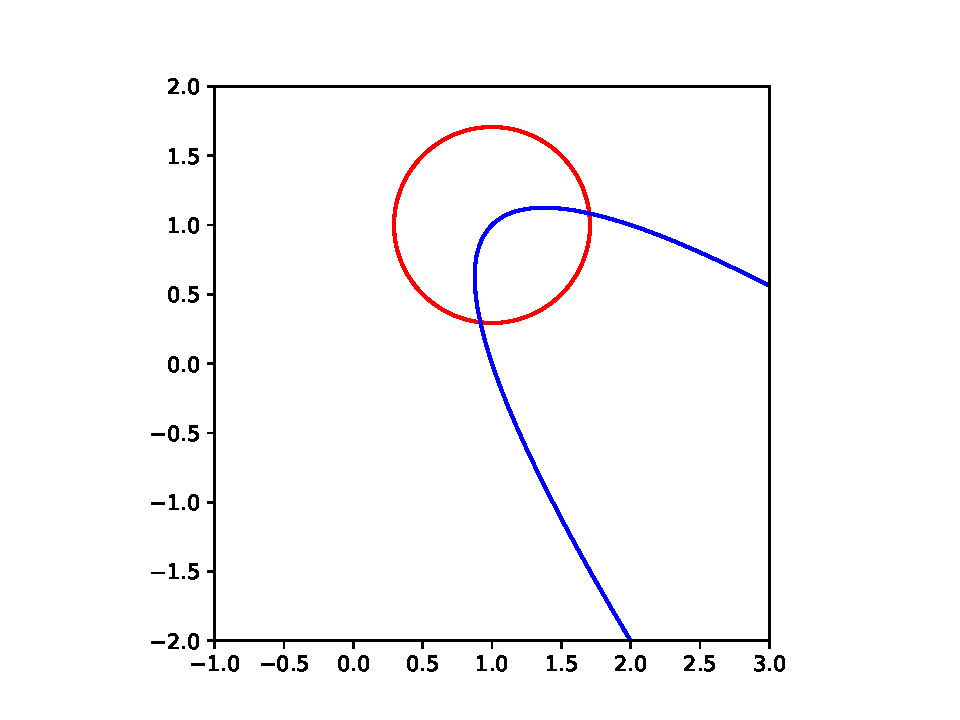
\includegraphics{math/fig/hw2/ex7.pdf}
    \caption{Ex 7.a: Zero contours of $p(x,y)$ (red) and $q(x,y)$ (blue)}
    \label{fig:ex7a}
\end{figure}

\subexercise
\begin{equation*}
    \begin{aligned}
        p(x,y) & = & 2y^2 & - 4y & + 2x^2 - 4x + 3 \\
        q(x,y) & = & y^2 & + (2x - 3) y & + x^2 - 5x + 4 
    \end{aligned}
\end{equation*}

So, we have
\begin{equation*}
\begin{aligned}
    \det(Q) & = \det \left(
        \begin{array}{cccc}
        2 & -4 & 2x^2 - 4x + 3 & 0  \\
        0 & 2 & -4 & 2x^2 - 4x + 3  \\
        1 & 2x - 3 & x^2 - 5x + 4 & 0  \\
        0 & 1 & 2x - 3 & x^2 - 5x + 4  \\
    \end{array}
    \right) \\
    & (\text{subtract the 3rd row twice from the 1st row,} \\ & \text{this does \textbf{not} change the value of determinant}) \\
    & = \det \left(
        \begin{array}{cccc}
        0 & -4x+2 &  6x - 5 & 0  \\
        0 & 2 & -4 & 2x^2 - 4x + 3  \\
        1 & 2x - 3 & x^2 - 5x + 4 & 0  \\
        0 & 1 & 2x - 3 & x^2 - 5x + 4  \\
    \end{array}
    \right) \\
    & = \det \left(
        \begin{array}{ccc}
        -4x+2 &  6x - 5 & 0  \\
        2 & -4 & 2x^2 - 4x + 3  \\
        1 & 2x - 3 & x^2 - 5x + 4  \\
    \end{array}
    \right) \\
    & = (-4x+2) \det \left(
        \begin{array}{cc}
         -4 & 2x^2 - 4x + 3  \\
         2x - 3 & x^2 - 5x + 4  \\
    \end{array}
    \right)
    - (6x-5) \det \left(
        \begin{array}{cc}
         2 & 2x^2 - 4x + 3  \\
         1 & x^2 - 5x + 4  \\
    \end{array}
    \right)\\
    & = (-4x+2)(-4(x^2 - 5x + 4) - (2x - 3)(2x^2 - 4x + 3)) \\
     & \quad - (6x - 5)(2(x^2 - 5x + 4) - (2x^2 - 4x + 3)) \\
    & =(-4x+2)(-4x^2 + 20x - 16 - (4x^3 - 8x^2 + 6x - 6x^2 + 12x - 9)) \\
    & \quad - (6x - 5)(2x^2 - 10x + 8 - 2x^2 + 4x - 3) \\
    & = (-4x+2)(-4x^3+10x^2+2x-7) - (6x-5)(-6x+5) \\
    & = 16x^4 - 48x^3 + 12x^2 + 32x - 14 + 36x^2 - 60x + 25 \\
    & = 16x^4 - 48x^3 + 48x^2 - 28x + 11.
\end{aligned}

\end{equation*}

Then I use $numpy.roots$ to solve this polynomial equation $16x^4 - 48x^3 + 48x^2 - 28x + 11 = 0$. The real roots are $x_1 = 1.702, x_2 = 0.916$.

When $x_1 = 1.702$, $y_1 = (-1)^{1+2} \frac{\det(Q_1)}{\det(Q_2)} = 1.084$.

When $x_2 = 0.916$, $y_1 = (-1)^{1+2} \frac{\det(Q_1)}{\det(Q_2)} = 0.299$.

\subexercise
In Fig \ref{fig:ex7c}, I plot these 2 points $(1.702, 1.084)$ and $(0.916, 0.299)$ on the sketch. Clearly, they're located on the intersection points.

\begin{figure}
    \centering
    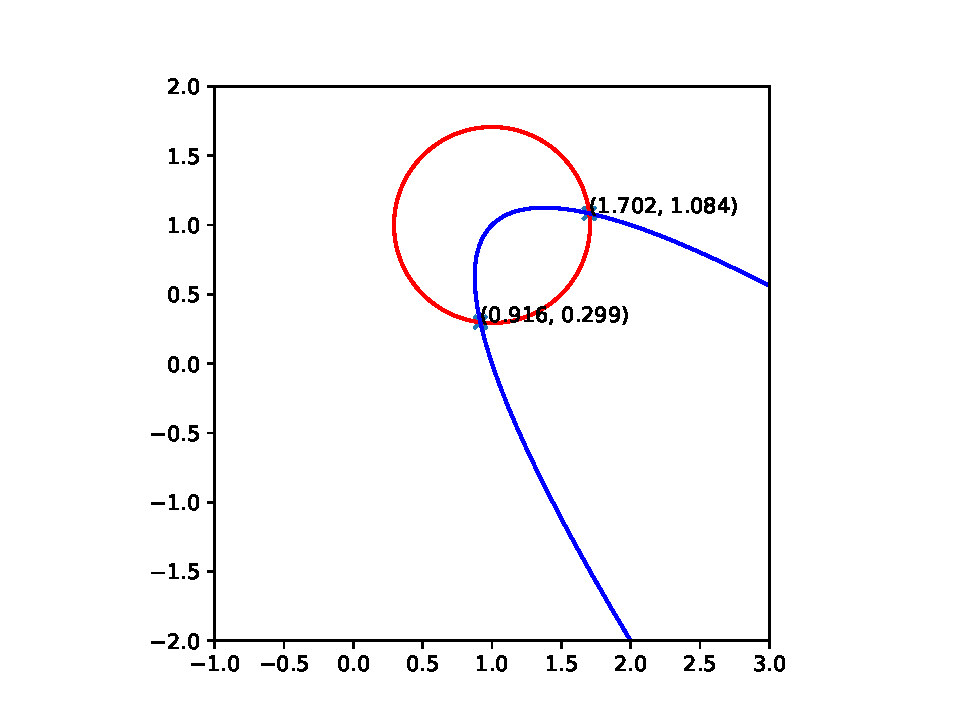
\includegraphics{math/fig/hw2/ex7c.pdf}
    \caption{Ex 7.c: Visualization of 2 roots.}
    \label{fig:ex7c}
\end{figure}

\exercise
\subexercise
Let $\Vec{w_i} = (x^{(i)}, y^{(i)})$, and the same for $j, k$. Let $\Vec{w} = (x, y)$. Consider dividing the vector $\Vec{w} - \Vec{w_i}$ into 2 bases: $(\Vec{w_j} - \Vec{w_i})$ and $(\Vec{w_k} - \Vec{w_i})$. This can be formulated as:

\begin{equation}
    \Vec{w} - \Vec{w_i} = a \cdot (\Vec{w_j} - \Vec{w_i}) + b \cdot (\Vec{w_k} - \Vec{w_i}).
\label{eq:ex8a1} 
\end{equation}

In this sense, the point $(x, y)$ falls within the triangle 

\noindent $\Leftrightarrow 0 \le a \le 1$ and $0 \le b \le 1$ and $a + b \le 1$.

On the other hand, we can reformulate Eq. \ref{eq:ex8a1} as:
\begin{equation*}
    (\Vec{w_j} - \Vec{w_i}, \Vec{w_k} - \Vec{w_i}) \cdot \left(
        \begin{array}{c}
         a \\
         b
    \end{array}
    \right) = \Vec{w} - \Vec{w_i}.
\end{equation*}

In other words,
\begin{equation}
    \left(
        \begin{array}{cc}
         x^{(j)} - x^{(i)} & x^{(k)} - x^{(i)} \\
         y^{(j)} - y^{(i)} & y^{(k)} - y^{(i)}
    \end{array}
    \right) \cdot
    \left(
    \begin{array}{c}
         a \\
         b
    \end{array}
    \right) =
    \left(
    \begin{array}{c}
        x - x^{(i)} \\
        y - y^{(i)}
    \end{array}
    \right)
\label{eq:ex8a2}
\end{equation}

Therefore, to determine whether a point $(x,y)$ falls within the triangle, we first solve the System (\ref{eq:ex8a2}). If $0 \le a \le 1$ and $0 \le b \le 1$ and $a + b \le 1$, then the point falls within the triangle. Otherwise not.

\subexercise
I implement this algorithm in $ex8.py$. The script takes 2 float as input (the starting point), and will output a figure specifies the interpolated path.

\subexercise Below are several topics when implementing the algorithm.

\begin{itemize}
    \item \noindent \textbf{How to identify which side of the ring a path lies on:} The idea is to see whether most points on the path are on either side of the line $y=x$. Specifically, for each path $p^{(i)}$, calculate $\sum \limits_{l=0}^{49} (x^{(i)}_l - y^{(i)}_l)$. If that value is less than or equals to $0$, than the path lies on the upper side of the ring. Otherwise, the path lies on the bottom side of the ring.
    
    \item \noindent \textbf{Pick of $p^{(i)},p^{(j)}$ and $p^{(k)}$:} Iterate all the triplets $(i,j,k)$ in the range of $0,1,2,\cdots,n-1$ with the restrict that $i < j < k$. For each triplet $(i, j, k)$, first check if these 3 paths lie on the same side of the ring. Then check if $p(0)$ falls within the triangle formed by the starting locations of these 3 paths. Finally, calculate the sum of distances from $p(0)$ to the starting locations of these 3 paths. Pick such 3 paths that have the smallest sum of distances.
    
    \item \noindent \textbf{Calculation of $\alpha_i, \alpha_j$ and $\alpha_k$:} From Eq.\ref{eq:ex8a1}, we have $\Vec{w} = (1-a-b) \cdot\Vec{w_i} + a \cdot \Vec{w_j} + b \cdot \Vec{w_k}.$ Then we can assign: $\alpha_i = 1-a-b, \alpha_j = a, \alpha_k=b$, where $a$ and $b$ can be obtained during the checking process of triangle. The advantage of this assignment is that we have $0 \le \alpha_i \le 1, 0 \le \alpha_j \le 1, 0 \le \alpha_k \le 1$, which makes the weights more average. This makes the weighted sum path more stable.
    
    \item \noindent \textbf{Interpolation:} For $t \in [i,i+1]$, I interpolate the path using 3 points $t = i-1, i, i+1$. Exceptionally, for $t \in [0,1]$, I interpolate the path using $t = 0, 1, 2$.
    Using 3 points is smoother than using merely 2 points (linear interpolation). Considering it is under a scene of a circus act, the algorithm should be real-time and runs very quickly. Quadratic interpolation consumes less time than using more points. So I choose quadratic interpolation as the method. In implementation, I reuse my code on interpolation in $ex1.py$.
    
    \item \noindent \textbf{Time scale:} I choose $0.01$ as the time step when interpolating the path.
\end{itemize}

\subexercise
Fig. \ref{fig:ex8d1}, \ref{fig:ex8d2} and \ref{fig:ex8d3} show the result. The 3 paths being interpolated are shown by green lines. The weighted sum points of the calculated path are shown by yellow crosses. The interpolated path is shown by blue lines. The ring of fire is shown by the red circle.


\begin{figure}
    \centering
    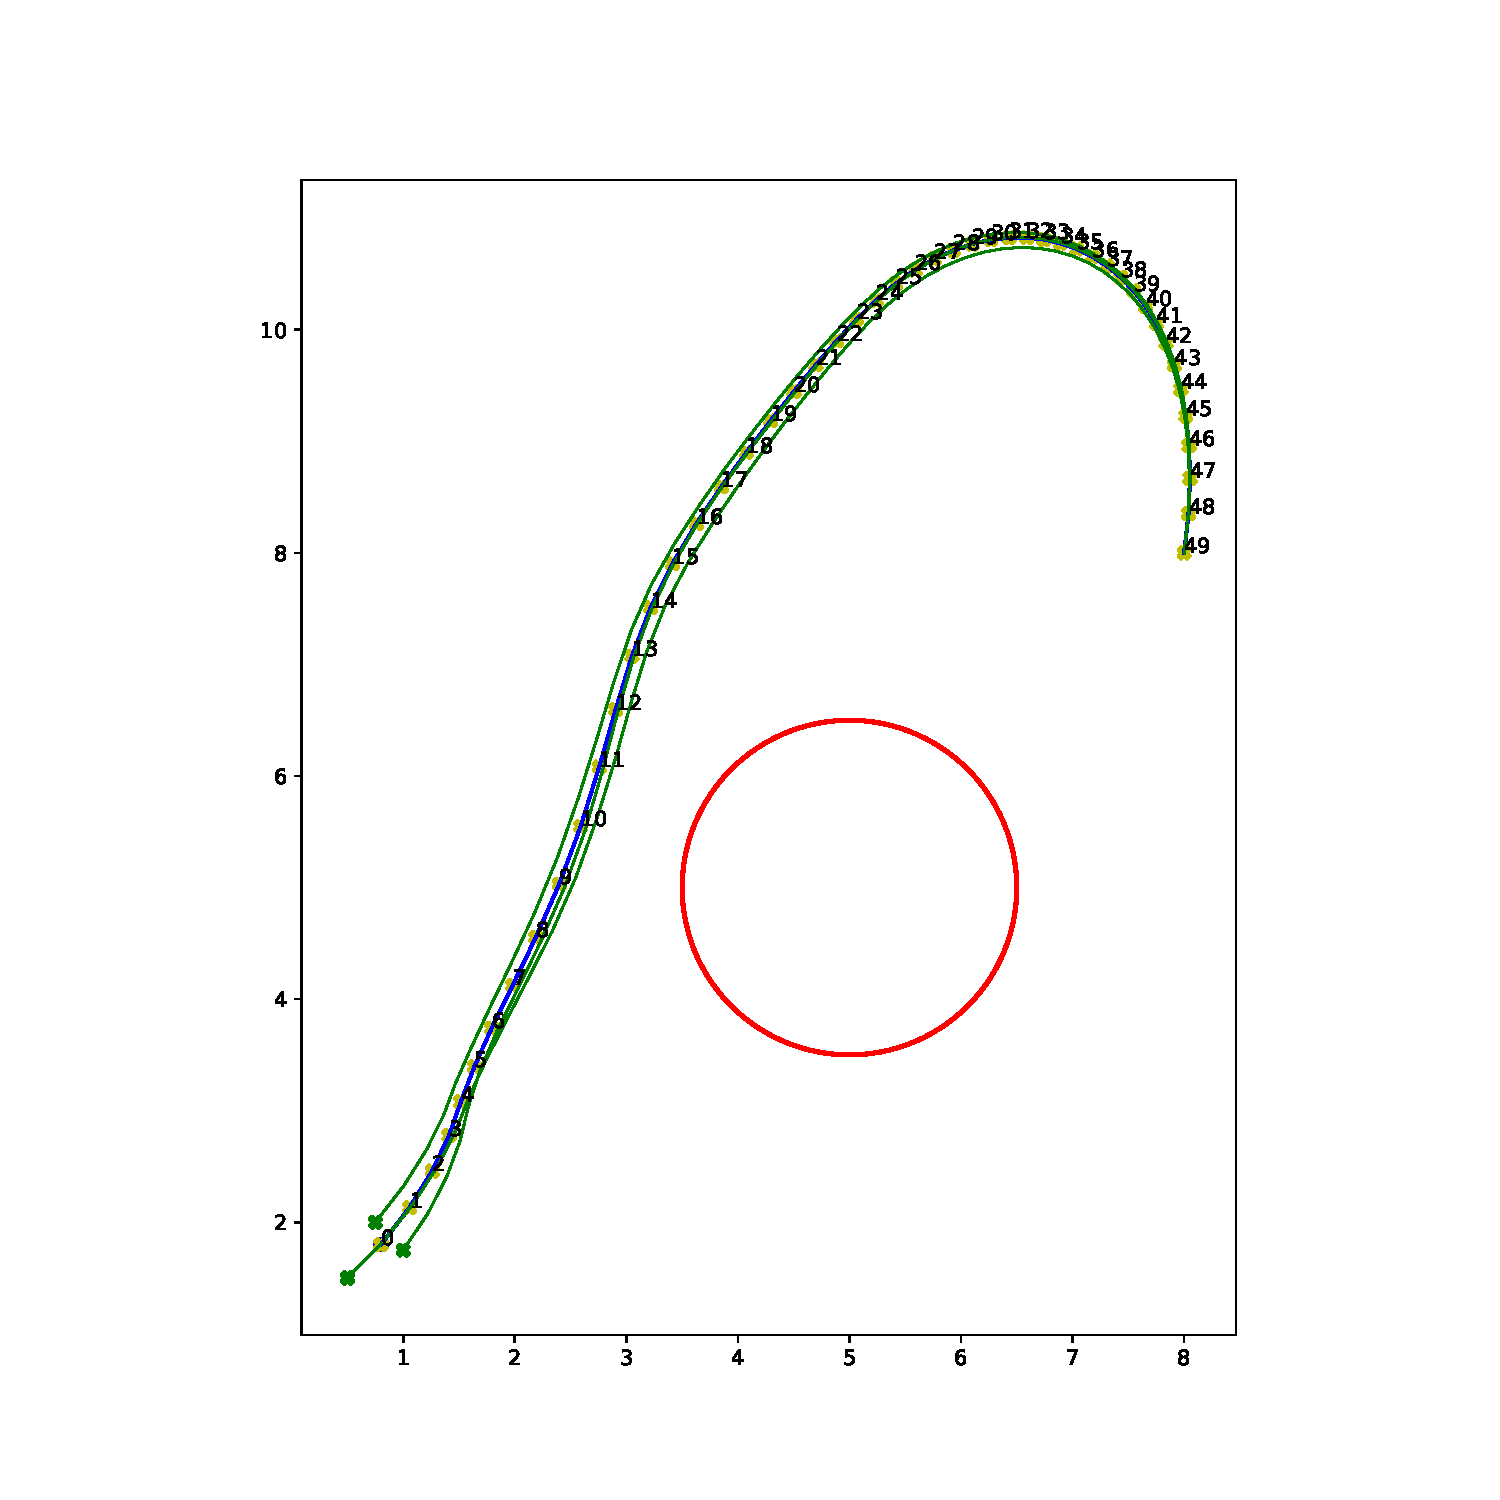
\includegraphics[width=\linewidth]{math/fig/hw2/ex8c1.pdf}
    \caption{Ex 8.d Starting Point: (0.8, 1.8)}
    \label{fig:ex8d1}
\end{figure}

\begin{figure}
    \centering
    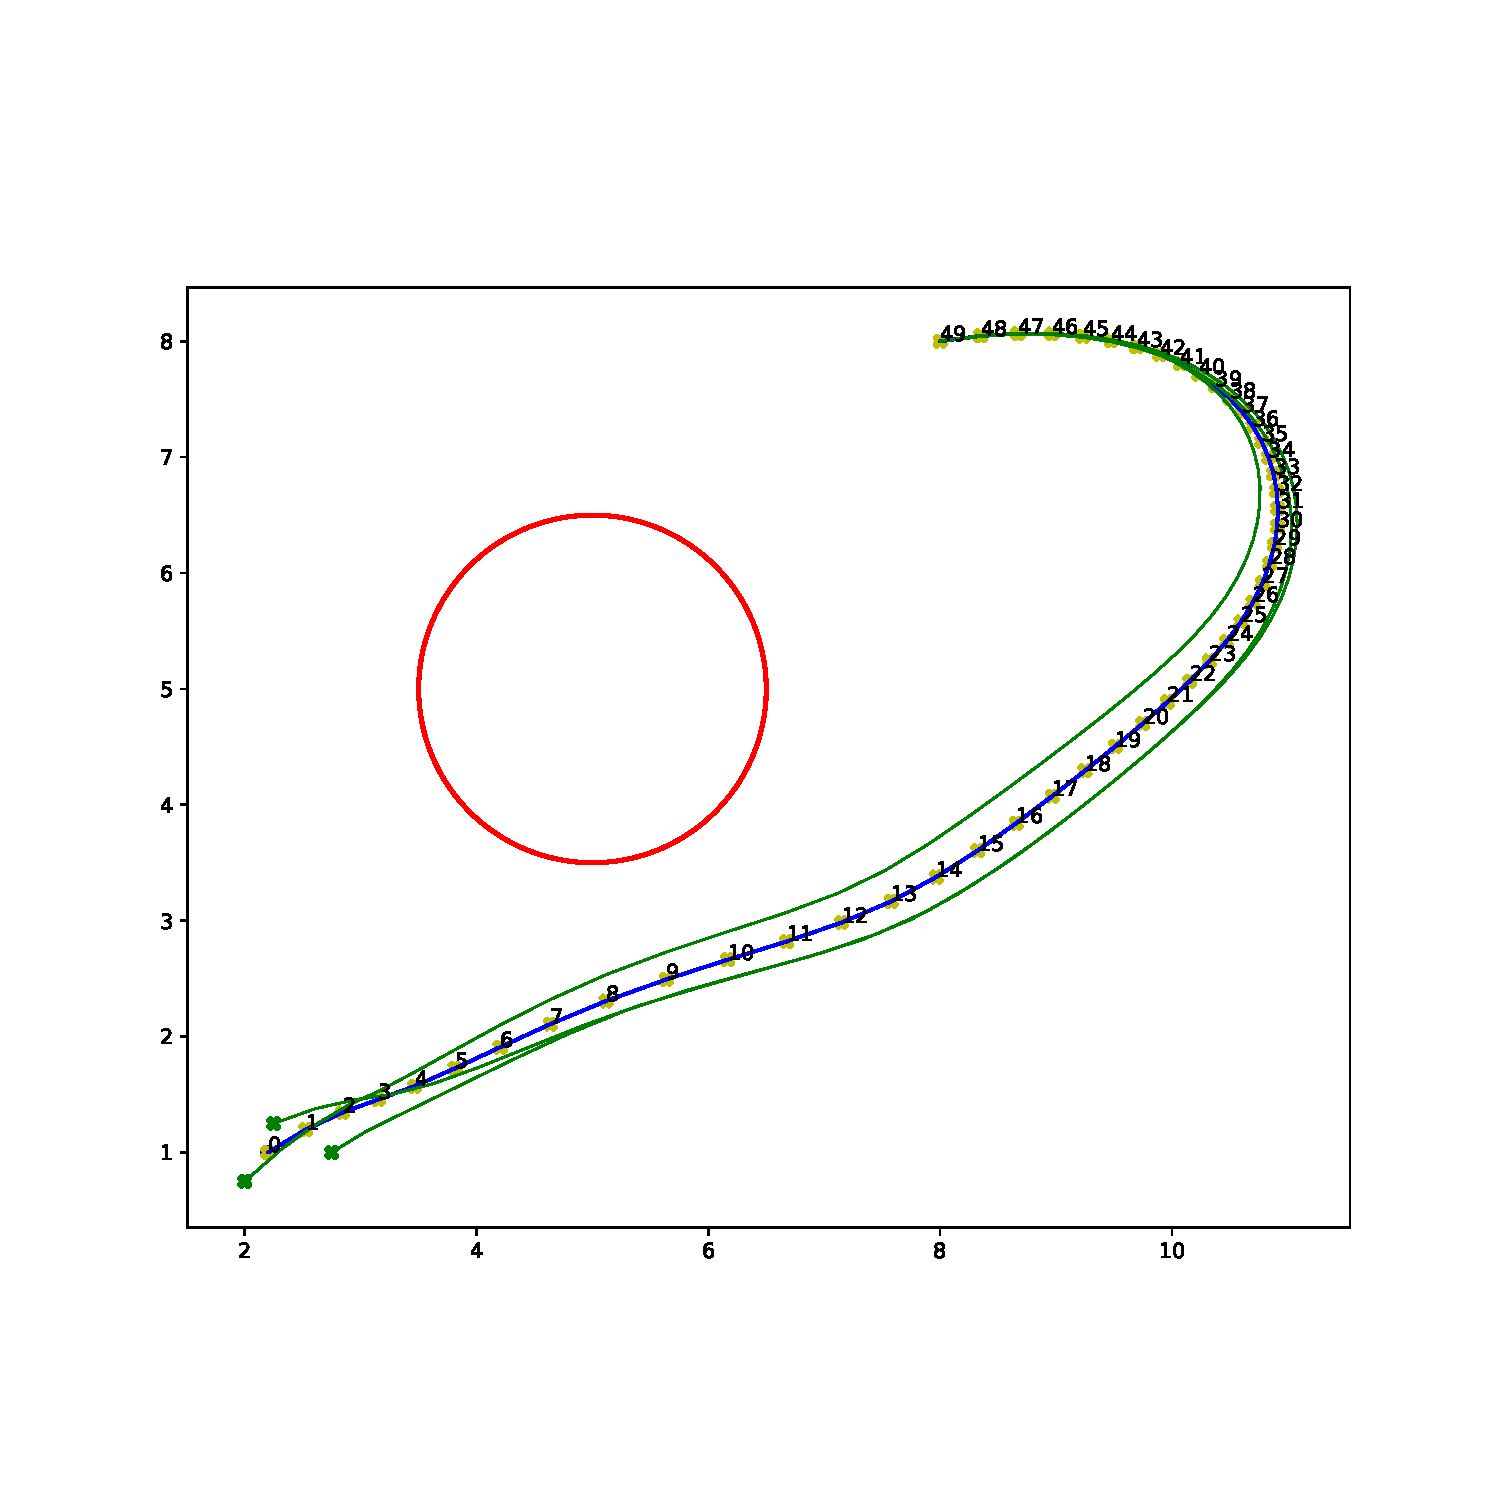
\includegraphics[width=\linewidth]{math/fig/hw2/ex8c2.pdf}
    \caption{Ex 8.d Starting Point: (2.2, 1.0)}
    \label{fig:ex8d2}
\end{figure}

\begin{figure}
    \centering
    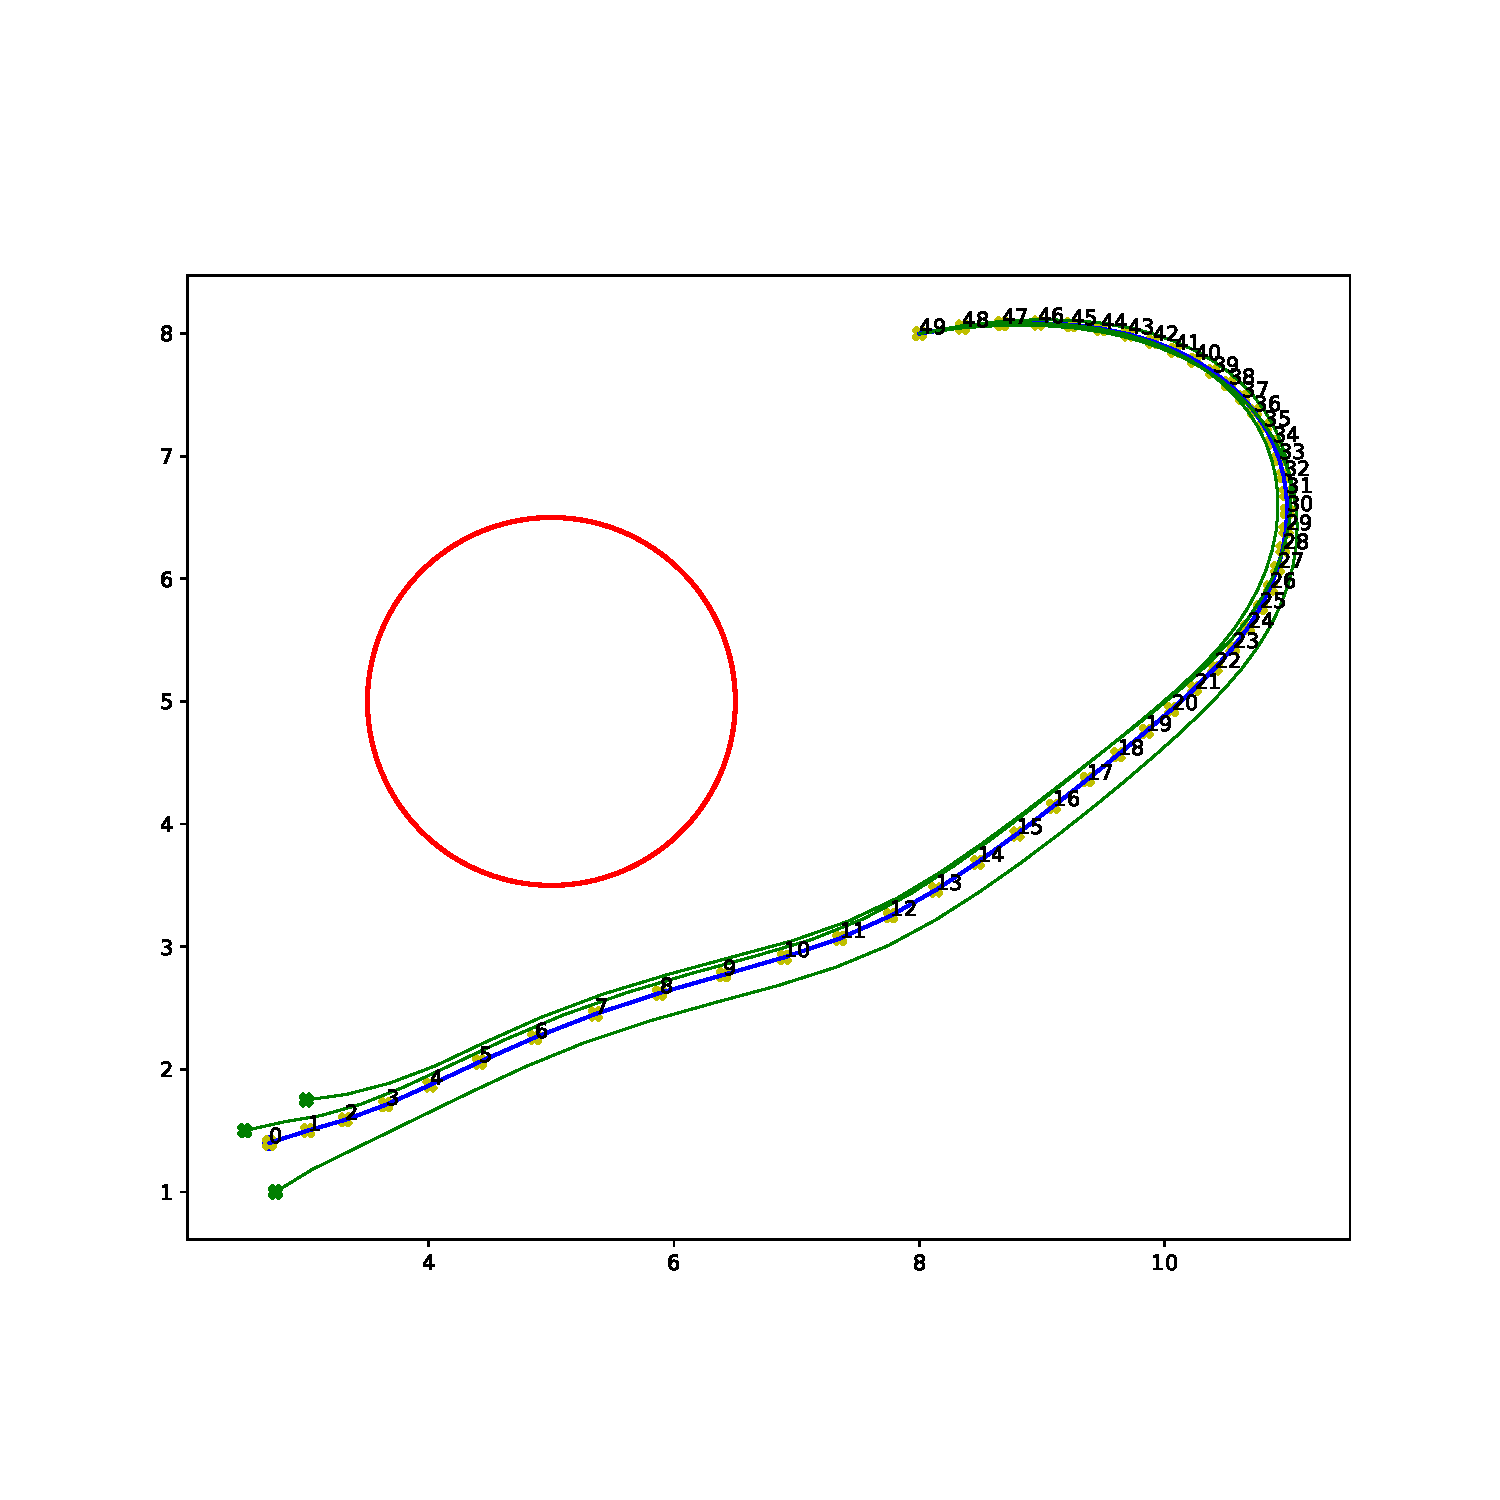
\includegraphics[width=\linewidth]{math/fig/hw2/ex8c3.pdf}
    \caption{Ex 8.d Starting Point: (2.7, 1.4)}
    \label{fig:ex8d3}
\end{figure}

\subexercise
If more obstacles were to be introduced, the algorithm should be more careful when interpolating the path. The current algorithm guarantees that on each time snapshot, the new path falls within the triangle of those 3 pre-computed paths. In the current case, the pre-computed paths are far away from the ring. So there is no danger in interpolating the path. But with more obstacles, especially those are near the pre-computed paths, the algorithm should check if the interpolated path still does not touch the obstacles. To avoid touching obstacles, we can first interpolate those 3 pre-computed paths to make them more fine on time resolution, and re-compute the new path.


\end{document}
